\documentclass[a4paper]{article}

%% Language and font encodings
\usepackage[english]{babel}
\usepackage[utf8x]{inputenc}
\usepackage[T1]{fontenc}

%% Sets page size and margins
\usepackage[a4paper,top=3cm,bottom=2cm,left=3cm,right=3cm,marginparwidth=1.75cm]{geometry}

%% Useful packages
\usepackage{amsmath}
\usepackage{graphicx}
\usepackage[colorinlistoftodos]{todonotes}
\usepackage[colorlinks=true, allcolors=blue]{hyperref}
\usepackage{alltt}

\title{Reporte de Actividad 10}
\author{Valenzuela Terán Jonás}

\begin{document}
\maketitle


\begin{center}

	
\includegraphics[height=6cm]{logistic-bifurcation.png}

\end{center}

\section{Introducción}

La teoría del caos es una rama de las matemáticas que trata sistemas dinámicos no lineales, el propósito de la actividad es explorar el sistema de crecimiento de una población, a través de wxmaxima y gnuplot, donde se producen gráficos que ayudan a visualizar la naturaleza del sistema y los patrones que emergen de lo que a simple vista parece aleatoridad.

Estos pueden surgir de reglas simples, pero sus efectos se suman a producir un comportamiento caótico, además, son muy sensibles a las condiciones iniciales. Se basó la actividad del blog creado por Geoff Boeing donde implementó el ejemplo en python.

\section{La teoría del caos}

Nos basaremos de una función que describe como una población evoluciona con el tiempo, es una ecuación diferencial que considera al tiempo continuo, pero podemos trabajar su la forma discreta, con pequeños pasos en el tiempo:

\begin{center}
$x_{t+1}=rx_t (1- x_t)$
\end{center}

Donde $x$ representa la población en un tiempo t, y r representa la tasa de crecimiento. Si r es muy bajo, la población no es capaz de sobrevivir y se extingue, si es muy alta, la población puede tender a un valor o oscilar entre caídas y aumentos.

Puede parecer simple, pero con ciertos valores de la tasa de crecimiento, se produce un sistema caótico, para ciertos valores es posible distinguir atractores, valores a los que tiende la población. Si analizamos diferentes tasas de crecimiento, se puede observar que aumenta el número de atractores al con tasas grandes, de modo que forman fractales al analizar como cambia el número de cerca, más adelante podremos apreciar lo mencionado con los gráficos obtenidos.

Además, podemos analizar una gráfica de fase, comparando los valores de la población en un tiempo $t+1$ contra $t$, lo que revela oscilaciones para el atractor de tasas de crecimiento entre 3 y 4.

\section{Implementación en wxmaxima}

Con ayuda del artículo "Chaotic dynamics with Maxima" por A. Morante, J.A. Vallejo, se producieron valores del modelo con tasas de crecimiento desde 0.5 a 3.5, utiliza la función "evolution", que al especificar la función, parámetros, valores iniciales y límites, resuelve la ecuación diferencial planteada del sistema y genera los datos.

\begin{center}
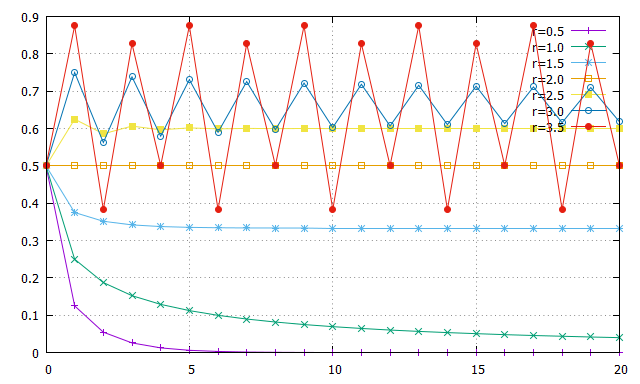
\includegraphics[height=7cm]{Grafica_Compilacion_1.png}
\end{center}

Para analizar los atractores de cada tasa de crecimiento en un rango amplio, utilizamos la función orbits, que nos permite tomar el ciclo límite de cada caso de evolución, con un rango para r. Produce valores estables para tasas de crecimiento reducidas, pero a partir de tasas alrededor de 3.5, ocurre una bifurcación que se acentúa cada vez más. Cada evolución fue guardada en archivos, para posteriormente ser graficados en gnuplot.

\begin{center}
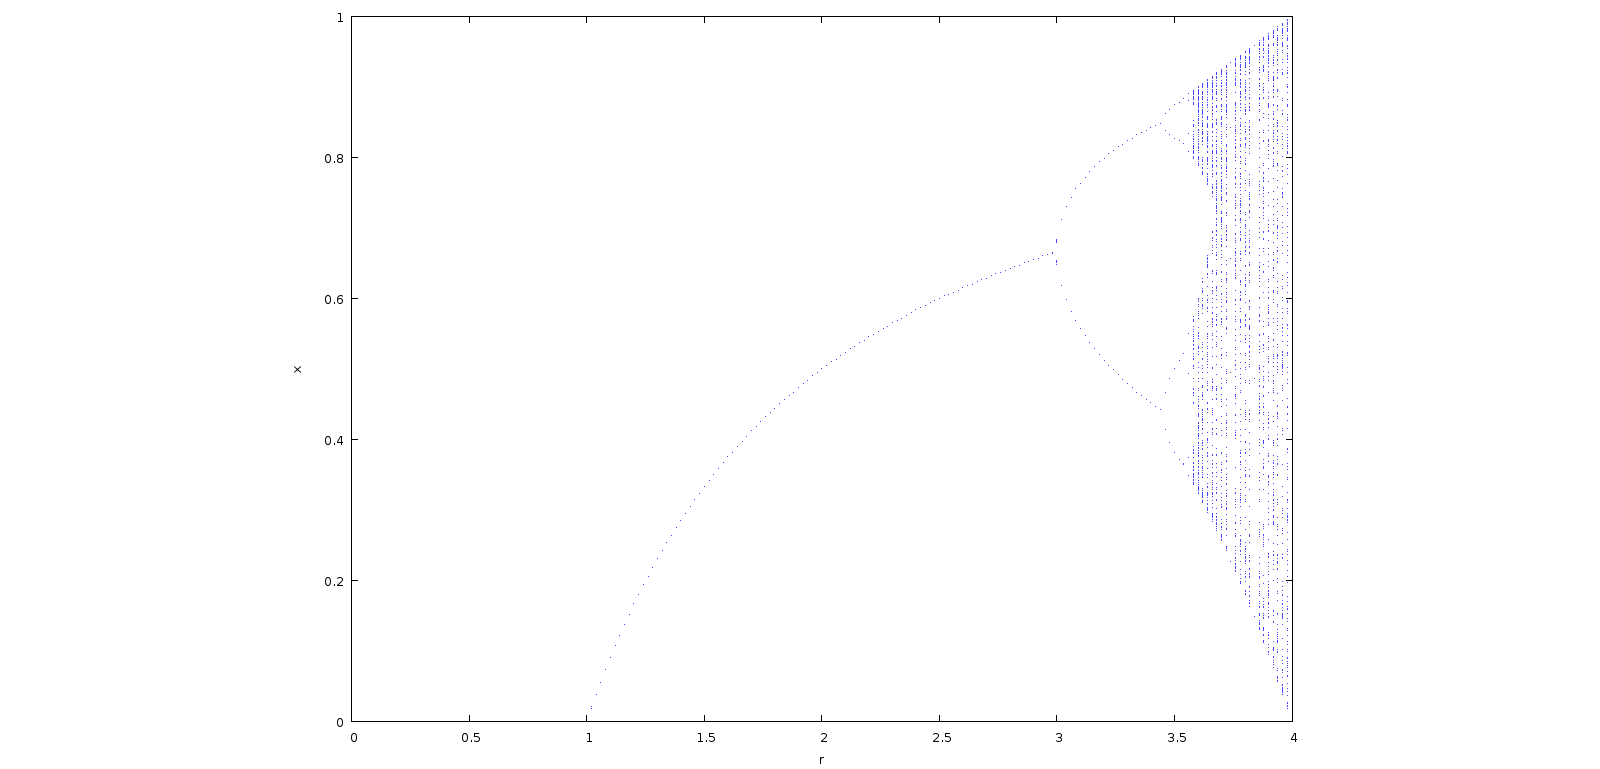
\includegraphics[height=6cm]{grafica3-1.png}
\end{center}

\begin{center}
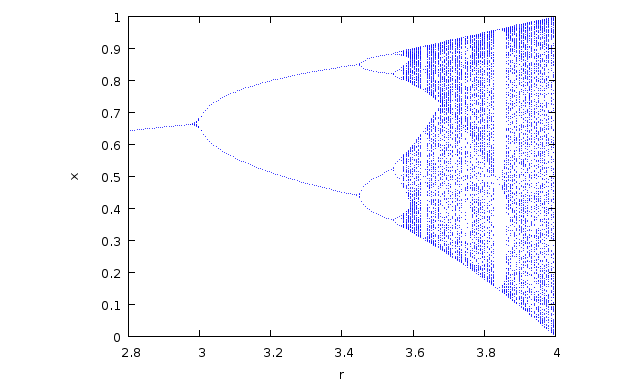
\includegraphics[height=6cm]{grafica3-2.png}
\end{center}

Si vemos suficientemente cerca una región de la bifurcación, podemos observar el mismo patrón del que se ve al observar todos los datos, creando un fractal.

\begin{center}
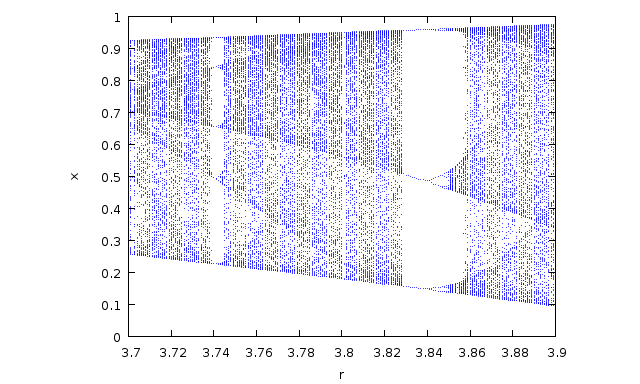
\includegraphics[height=6cm]{grafica3-3.png}
\end{center}

\begin{center}
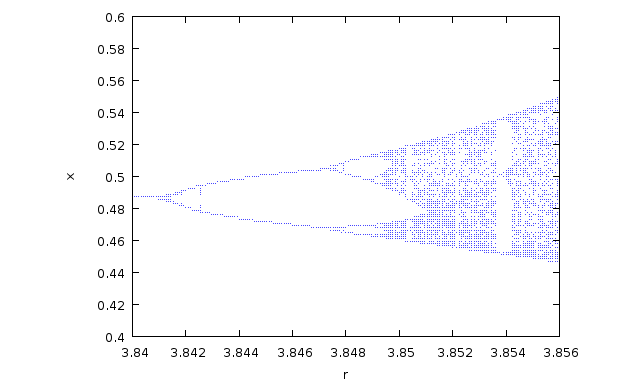
\includegraphics[height=6cm]{grafica3-4.png}
\end{center}

Para observar las gráficas de fase, se generaron datos con la función "evolution" para tasas de crecimiento de 3.6 a 4, y se guardaron en archivos para poder generar datos comparando la población $t+1$ y $t$, acomodando cada uno en una columna. 

Estos se graficaron en gnuplot, ya que maxima usa gnuplot para sus gráficas, y da más opciones y mejores resultados usar gnuplot directamente.

\begin{center}
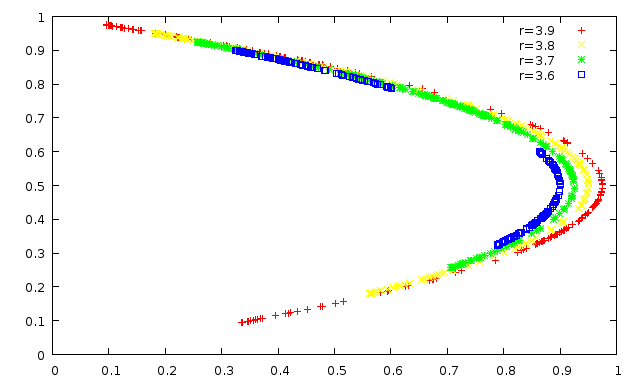
\includegraphics[height=6cm]{Grafica_Compilacion_2.png}
\end{center}

Los datos describen parábolas, pero curiosamente, ningún atractor se repite, siempre oscila entre diferentes valores de población, esto solo es cierto para valores de tasa de crecimiento en estos rangos, para valores pequeños, solo un conjunto de puntos se repiten.


\section{Conclusión}

Poseemos muchas herramientas para describir sistemas y resolver problemas relacionados a ellos, en este caso, usamos wxmaxima para reproducir algo que se hizo en python, eso muestra la flexibilidad y la gran cantidad de alcance que tienen. Además, aprendimos un poco del caos, como de reglas simples surgen sistemas que parecen aleatorios, pero a través del análisis de datos se encuentran patrones muy interesantes.

\section{Bibliografía}

Geoff Boeing. (2015). Chaos Theory and the Logistic Map. 10 de mayo 2018, de UC Berkeley Sitio web: \textit{http://geoffboeing.com/2015/03/chaos-theory-logistic-map/}

A. Morante and J. A. Vallejo. (2013). Chaotic dynamics with Maxima. 10 de mayo 2018, de Universidad Autónoma de San Luis Potosí Sitio web: https://arxiv.org/pdf/1301.3240.pdf


\end{document}